%\pdfoutput=1 % to force arxiv to use pdflatex
%\documentclass[prl,twocolumn,superscriptaddress]{revtex4-1}
%\documentclass[prl,fourcolumn,superscriptaddress]{revtex4-1}
%\documentclass[prl,precolumn, superscriptaddress]{revtex4-1}
\documentclass[prl,onecolumn, superscriptaddress]{revtex4-1}

\usepackage{geometry}
\usepackage{lipsum}
\geometry{
  paperwidth=150mm,     % Largeur de la page
  %paperheight=345mm,    % Hauteur de la page
  paperheight=200mm,    % Hauteur de la page
  %paperheight=5000mm,  % Hauteur de la page
  textwidth=100mm,      % Largeur du texte
  textheight=230mm,     % Hauteur du texte
  left=2mm,            	% Marge gauche
  right=2mm,			% Marge droite
  top=2mm,             	% Marge supérieure
  bottom=2mm,			% Marge inférieure
}


\usepackage{graphicx}
\usepackage{color}
\usepackage{amssymb}
\usepackage{bm}
\usepackage{amsmath,amsfonts,latexsym}

% Ajouter ce package pour redéfinir la taille de la police
%\usepackage{anysize}
\usepackage{setspace}
% Changer la taille de la police pour tout le document
\renewcommand{\normalsize}{\fontsize{18}{10}\selectfont}
%\renewcommand{\normalsize}{\fontsize{2}{1}\selectfont}


% Définir une couleur grise personnalisée
%\definecolor{mygray}{gray}{0.3}
%\definecolor{myred}{rgb}{0.5, 0, 0}

\definecolor{tradcolor}{rgb}{0, 0, 0.5}
\definecolor{resumecolor}{rgb}{0.5, 0, 0}

% Nouvelle commande pour les traductions
%\newcommand{\trad}[1]{\textcolor{mygray}{#1}}
\newcommand{\trad}[1]{\textcolor{tradcolor}{#1}}

%\newcommand{\resumefr}[1]{\textcolor{myred}{#1}}
\newcommand{\resumefr}[1]{\textcolor{resumecolor}{#1}}

\usepackage{braket} % For bra-ket notation
\usepackage{enumitem}
%\usepackage{array,tabularx}
%\usepackage{dcolumn}               % Align table columns on decimal
%\usepackage{groupedaddress}				% point

%\usepackage{hyperref}              %don't get compounds citations e.g. [1-5]
\usepackage{comment}

\usepackage{bm} % allows bold greek letters

\newcommand*{\br}{\mathbf{r}}
\newcommand*{\bp}{\mathbf{p}}
\newcommand*{\bk}{\mathbf{k}}
\newcommand*{\bq}{\mathbf{q}}
\newcommand*{\bv}{\mathbf{v}}
\newcommand*{\cA}{{\cal A}}
\newcommand*{\cB}{{\cal B}}
\newcommand*{\cD}{{\cal D}}
\newcommand*{\cF}{{\cal F}}
\newcommand*{\cC}{{\cal C}}
\newcommand*{\cE}{{\cal E}}
\newcommand*{\cZ}{{\cal Z}}
\newcommand*{\cN}{{\cal N}}
\newcommand*{\cL}{{\cal L}}
\newcommand*{\cH}{{\cal H}}
\newcommand*{\cT}{{\cal T}}
\newcommand*{\cY}{{\cal Y}}
\newcommand*{\cV}{{\cal V}}
\newcommand*{\cQ}{{\cal Q}}
\newcommand*{\cI}{{\cal I}}
\newcommand*{\cP}{{\cal P}}
\newcommand*{\cR}{{\cal R}}
\newcommand*{\cM}{{\cal M}}

\newcommand*{\pop}{\psi^{\vphantom{\dagger}}}
\newcommand*{\pdop}{\psi^\dagger}
\newcommand*{\Phop}{\Phi^{\vphantom{\dagger}}}
\newcommand*{\Phdop}{\Phi^\dagger}
\newcommand*{\phop}{\phi^{\vphantom{\dagger}}}
\newcommand*{\phdop}{\phi^\dagger}
\newcommand*{\aop}{a^{\vphantom{\dagger}}}
\newcommand*{\adop}{a^\dagger}
\newcommand*{\bop}{b^{\vphantom{\dagger}}}
\newcommand*{\bdop}{b^\dagger}
\newcommand*{\cop}{c^{\vphantom{\dagger}}}
\newcommand*{\cdop}{c^\dagger}

\newcommand*{\sgn}{\mathrm{sgn}}

\DeclareMathOperator{\tr}{tr}
\newcommand{\vect}[1]{\bm{#1}}

\begin{document}

\title{From GPE to KPZ: finite temperature dynamical structure factor of the 1D Bose gas \\ \trad{De l'équation de Gross-Pitaevskii (GPE) à l'équation de Kardar-Parisi-Zhang (KPZ) : facteur de structure dynamique à température finie du gaz de Bose en 1D.}}
\author{Manas Kulkarni}
\affiliation{Department of Physics, University of Toronto, Ontario, M5S 1A7, Canada}
\affiliation{Department of Physics, University of Virginia,
Charlottesville, VA 22904-4714 USA}
\author{Austen Lamacraft} 
\affiliation{Department of Physics, University of Virginia,
Charlottesville, VA 22904-4714 USA}
\date{\today}
%\email{austen@virginia.edu} 
\date{\today}

\begin{abstract}

We study the finite temperature dynamical structure factor $S(k,\omega)$ of a 1D Bose gas using numerical simulations of the Gross--Pitaevskii equation appropriate to a weakly interacting system. The lineshape of the phonon peaks in $S(k,\omega)$ has a width $\propto |k|^{3/2}$ at low wavevectors. This anomalous width arises from resonant three-phonon interactions, and reveals a remarkable connection to the Kardar--Parisi--Zhang universality class of dynamical critical phenomena.\\
\trad{Nous étudions le facteur de structure dynamique à température finie $S(k,\omega)$ d'un gaz de Bose unidimensionnel en utilisant des simulations numériques de l'équation de Gross--Pitaevskii appropriée à un système faiblement interactif. La forme du pic des phonons dans $S(k,\omega)$ présente une largeur $\propto |k|^{3/2}$ pour de faibles vecteurs d'onde. Cette largeur anormale provient des interactions résonantes à trois phonons et révèle une connexion remarquable avec la classe d'universalité Kardar--Parisi--Zhang des phénomènes critiques dynamiques.
}
\end{abstract}

\maketitle

The statistical mechanics of low dimensional fluids, both quantum and classical, has long been a source of theoretical surprises. To give just two examples:
%
\begin{enumerate}[itemsep=2pt,parsep=1pt]
	\item The long-time tail $\propto t^{-d/2}$ in the velocity autocorrelation function of a $d$-dimensional classical fluid invalidates hydrodynamics for $d\leq 2$ \cite{Alder:1970,Ernst:1970,Dorfman:1970}.
	
	\item The Luttinger liquid description \cite{Haldane:1981} provides a universal language for 1D quantum liquids, with a panoply of phases arising upon perturbation \cite{Giamarchi:2004}. 
\end{enumerate}
%

\trad{
La mécanique statistique des fluides de basse dimension, tant quantiques que classiques, a longtemps été une source de surprises théoriques. Pour donner seulement deux exemples :
\begin{enumerate}[itemsep=2pt,parsep=1pt]
	\item La queue à long terme \(\propto t^{-d/2}\) dans la fonction d'autocorrélation de la vitesse d'un fluide classique en dimension \(d\) invalide l'hydrodynamique pour \(d\leq 2\) \cite{Alder:1970,Ernst:1970,Dorfman:1970}.	
	\item La description du liquide de Luttinger \cite{Haldane:1981} fournit un langage universel pour les liquides quantiques en 1D, avec une panoplie de phases émergeant sous perturbation \cite{Giamarchi:2004}.
\end{enumerate}
}

Despite these achievements recent developments in the theory of 1D quantum liquids away from the low energy limit make it clear that our understanding of these systems is still rather limited (for a review, see Ref.~\cite{Imambekov:2011}). To take a simple example, consider the dynamical structure factor $S(k,\omega)$ that gives the cross section for inelastic scattering from the liquid as a function of momentum $\hbar k$ and energy $\hbar\omega$ transferred. The Luttinger liquid theory predicts that $S(k,\omega)$ consists only of a pair of delta function peaks $\omega = \pm c|k|$, with $c$ the velocity of sound, corresponding to an undamped phonon oscillation.  At finite $k$, however, one expects this delta function to broaden due to interactions between phonons. Attempts to find the resulting lineshape using perturbation theory within the Luttinger framework are plagued by divergences \cite{Aristov:2007}, whose origin we will describe below. As a result, the possibility of capturing the relevant physics within the Luttinger or hydrodynamic formalism is now viewed with a degree of pessimism \cite{Cheianov:2009}.
\trad{Malgré ces réalisations, les développements récents de la théorie des liquides quantiques en 1D, au-delà de la limite basse énergie, montrent clairement que notre compréhension de ces systèmes est encore assez limitée (pour une revue, voir Ref.~\cite{Imambekov:2011}). Pour prendre un exemple simple, considérons le facteur de structure dynamique \(S(k,\omega)\), qui donne la section efficace de diffusion inélastique du liquide en fonction du moment \(\hbar k\) et de l'énergie \(\hbar\omega\) transférée. La théorie du liquide de Luttinger prédit que \(S(k,\omega)\) ne consiste qu'en une paire de pics de fonction delta \(\omega = \pm c|k|\), avec \(c\) la vitesse du son, correspondant à une oscillation de phonons non amortie. Cependant, pour un \(k\) fini, on s'attend à ce que cette fonction delta s'élargisse en raison des interactions entre phonons. Les tentatives pour trouver la forme de la ligne résultante en utilisant la théorie des perturbations dans le cadre de Luttinger sont perturbées par des divergences \cite{Aristov:2007}, dont nous décrirons l'origine ci-dessous. En conséquence, la possibilité de saisir la physique pertinente dans le formalisme de Luttinger ou hydrodynamique est maintenant perçue avec un certain pessimisme \cite{Cheianov:2009}.
}


Almost all of the developments reviewed in Ref.~\cite{Imambekov:2011} pertain to zero temperature. In this work we study the dynamical structure factor of a 1D Bose gas at finite temperature. Aside from being of paramount importance in real systems, we will show that finite temperature brings qualitatively new features that cannot be interpreted simply as a smearing of the zero temperature lineshape. Using analytical arguments and simulations of the Gross--Pitaevskii equation (GPE) appropriate to weak interactions and finite temperature $T$, we find that the lineshape of the phonon peak in $S(k,\omega)$ has a width $\Gamma_{k}\propto |k|^{3/2}$ at low $k$ (see Fig.~\ref{fig:Lineshape}). As well as dominating any zero temperature structure (generally $\propto k^{2}$) at low wavevectors, the $3/2$ power is \emph{anomalous} relative to the $k^{2}$ scaling that follows from linearized hydrodynamics \cite{Forster:1975}.
\trad{Presque tous les développements examinés dans la Ref.~\cite{Imambekov:2011} concernent la température nulle. Dans ce travail, nous étudions le facteur de structure dynamique d'un gaz de Bose en 1D à température finie. En plus d'être d'une importance capitale dans les systèmes réels, nous montrerons que la température finie apporte des caractéristiques qualitativement nouvelles qui ne peuvent pas être simplement interprétées comme un flou de la forme de ligne à température nulle. En utilisant des arguments analytiques et des simulations de l'équation de Gross--Pitaevskii (GPE) adaptées aux interactions faibles et à une température finie \(T\), nous trouvons que la forme de la ligne du pic de phonon dans \(S(k,\omega)\) présente une largeur \(\Gamma_{k}\propto |k|^{3/2}\) à faible \(k\) (voir Fig.~\ref{fig:Lineshape}). En plus de dominer toute structure à température nulle (généralement \(\propto k^{2}\)) à faible vecteur d'onde, la puissance de \(3/2\) est \emph{anormale} par rapport à la mise à l'échelle en \(k^{2}\) qui découle de l'hydrodynamique linéarisée \cite{Forster:1975}.
}

\begin{figure}
	\centering
	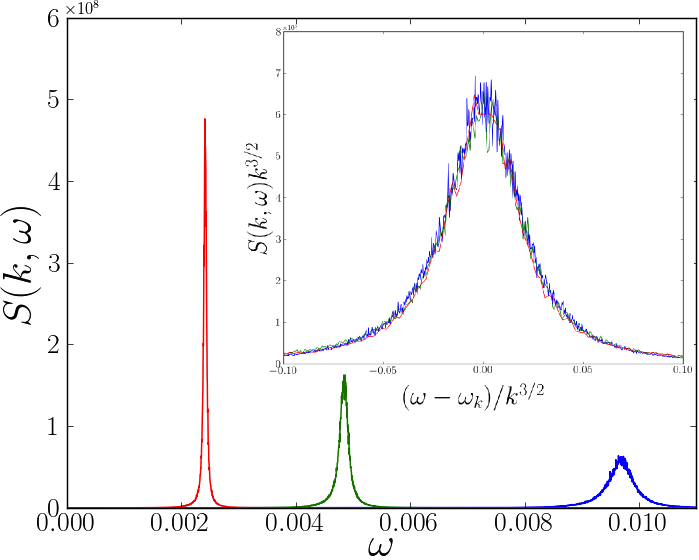
\includegraphics[width=\columnwidth]{RawAndScaled.png}
	\caption{Dynamical structure factor $S(k,\omega)$ of a 1D Bose gas described by the Gross--Pitaevskii equation for wavevectors $k=2\pi p/L$, $p=64,32,16$ (right to left). $L=5\times 2^{13}$ and temperature $T=0.005$, with length being measured in units of the healing length, and energy in units of the chemical potential. Inset: Scaling collapse of the phonon peaks using the ansatz Eq.~\eqref{GPEtoKPZ_PhononScaling}.\\
	\trad{Facteur de structure dynamique \(S(k,\omega)\) d'un gaz de Bose en 1D décrit par l'équation de Gross--Pitaevskii pour des vecteurs d'onde \(k=2\pi p/L\), avec \(p=64,32,16\) (de droite à gauche). \(L=5\times 2^{13}\) et température \(T=0.005\), les longueurs étant mesurées en unités de la longueur de guérison, et l'énergie en unités du potentiel chimique. Inset : Effondrement de l'échelle des pics de phonons utilisant l'ansatz Eq.~\eqref{GPEtoKPZ_PhononScaling}.
}}
	\label{fig:Lineshape}
\end{figure}


This unusual scaling points to a very rich phenomenology. According to a remarkable recent conjecture \cite{beijeren2011}, the long wavelength dynamics of a classical 1D fluid at finite temperature is in the Kardar--Parisi--Zhang (KPZ) universality class describing interface growth \cite{Kardar:1986,kriecherbauer2010,sasamoto2010}. Specifically, the phonon (Brillouin) peaks in $S(k,\omega)$ have the scaling form at low wavenumber
%
\begin{equation}
	\label{GPEtoKPZ_PhononScaling}
	S^{(\pm)}_{\text{phonon}}(k,\omega) \propto \frac{1}{\Gamma_{k}}f_{\text{PS}}\left(\frac{\omega\pm c|k|}{\Gamma_{k}}\right)
\end{equation}
%
where $f_{\text{PS}}(x)$ is given in Eq.~(5.7) of Ref.~\cite{prahofer2004}. The meaning of Eq.~\eqref{GPEtoKPZ_PhononScaling} is that in a frame moving at the speed of sound the density fluctuations moving in the same direction behave exactly as the fluctuations of the interface slope in the KPZ problem.

\trad{
Cette mise à l'échelle inhabituelle indique une phénoménologie très riche. Selon une conjecture remarquable récente \cite{beijeren2011}, la dynamique à longue longueur d'onde d'un fluide classique en 1D à température finie appartient à la classe d'universalité de Kardar--Parisi--Zhang (KPZ) décrivant la croissance des interfaces \cite{Kardar:1986,kriecherbauer2010,sasamoto2010}. Spécifiquement, les pics de phonons (Brillouin) dans \(S(k,\omega)\) ont la forme d'échelle suivante à faible nombre d'ondes :
\begin{equation*}
	%\label{GPEtoKPZ_PhononScaling}
	S^{(\pm)}_{\text{phonon}}(k,\omega) \propto \frac{1}{\Gamma_{k}}f_{\text{PS}}\left(\frac{\omega\pm c|k|}{\Gamma_{k}}\right)
\end{equation*}
où \(f_{\text{PS}}(x)\) est donné dans l'équation (5.7) de la Ref.~\cite{prahofer2004}. Le sens de l'équation \eqref{GPEtoKPZ_PhononScaling} est que dans un cadre se déplaçant à la vitesse du son, les fluctuations de densité se déplaçant dans la même direction se comportent exactement comme les fluctuations de la pente de l'interface dans le problème KPZ.
} 

There are very few experiments confirming KPZ scaling to date \cite{wakita1997,maunuksela1997,takeuchi2010}. Our hope is that the results of this Letter will lead to its observation in new systems. For example, the structure factor of 1D Bose gases of $^{87}$Rb was recently measured using Bragg spectroscopy \cite{Fabbri:2011}, while in Ref.~\cite{savard2011} the hydrodynamics of superfluid Helium in a single nanohole was investigated. In the latter case the sound absorption coefficient is presumably more accessible than the structure factor, and being $\propto\Gamma_{k}$ displays the same anomalous scaling.

\trad{
Il y a très peu d'expériences confirmant l'échelle KPZ à ce jour \cite{wakita1997,maunuksela1997,takeuchi2010}. Nous espérons que les résultats de cette Lettre conduiront à son observation dans de nouveaux systèmes. Par exemple, le facteur de structure des gaz de Bose en 1D de \(^{87}\)Rb a récemment été mesuré par spectroscopie de Bragg \cite{Fabbri:2011}, tandis que dans la Ref.~\cite{savard2011}, l'hydrodynamique de l'hélium superflu dans un seul nanohole a été étudiée. Dans ce dernier cas, le coefficient d'absorption acoustique est probablement plus accessible que le facteur de structure, et étant \(\propto \Gamma_{k}\), il affiche la même mise à l'échelle anormale.\\
}
%Bragg spectroscopy of atomic gases reviewed in Ref.~\cite{Ozeri:2005}



%The fundamental excitations of condensed matter systems are typically probed in inelastic scattering experiments. Measuring scattering as a function of momentum and energy transfer, assuming weak interaction between the scattered and scattering particles, yields the \emph{dynamic structure factor} $S(\mathbf{k},\omega)$. This is the Fourier transform of the density correlation function
%



\emph{Hydrodynamic description}. Our starting point is the \emph{classical} Hamiltonian describing a 1D gas of bosons of mass $m$ and interaction parameter $g$
%
\begin{equation}
	\label{GPEtoKPZ_GPHam}
	H = \int dx\,\left[\frac{|\partial_{x}\Psi|^{2}}{2m}+\frac{g}{2}|\Psi|^{4}\right],
\end{equation}
%
where the complex field $\Psi(x)$ obeys the Poisson bracket $\left\{\Psi^{\dagger}(x),\Psi(y)\right\}=i\delta(x-y)$, and we have set $\hbar=1$. The dynamics of $\Psi(x,t)$ is described by the familiar Gross--Pitaevskii equation. The mean field description embodied by the GPE is appropriate when the number of particles in a healing length $\xi\equiv\left(g\rho_{0}m\right)^{-1/2}$ is large, where $\rho_{0}$ denotes the mean density. This corresponds to `Luttinger parameter' $K\equiv\frac{\pi \rho_{0}}{mc}\gg 1$,  with $c=\sqrt{g\rho_{0}/m}$ the speed of sound in the uniform state.\\

\trad{
\emph{Description hydrodynamique}. Notre point de départ est le Hamiltonien \emph{classique} décrivant un gaz de bosons 1D de masse \(m\) et de paramètre d'interaction \(g\)
\begin{equation*}
	%\label{GPEtoKPZ_GPHam}
	H = \int dx\,\left[\frac{|\partial_{x}\Psi|^{2}}{2m}+\frac{g}{2}|\Psi|^{4}\right],
\end{equation*}
où le champ complexe \(\Psi(x)\) obéit à la relation de Poisson \(\left\{\Psi^{\dagger}(x),\Psi(y)\right\}=i\delta(x-y)\), et nous avons fixé \(\hbar=1\). La dynamique de \(\Psi(x,t)\) est décrite par l'équation de Gross--Pitaevskii familière. La description en champ moyen incarnée par l'équation de Gross--Pitaevskii est appropriée lorsque le nombre de particules dans une longueur de guérison \(\xi\equiv\left(g\rho_{0}m\right)^{-1/2}\) est grand, où \(\rho_{0}\) désigne la densité moyenne. Cela correspond au `paramètre de Luttinger' \(K\equiv\frac{\pi \rho_{0}}{mc}\gg 1\), avec \(c=\sqrt{g\rho_{0}/m}\) la vitesse du son dans l'état uniforme.
} 

After writing the condensate order parameter as $\Psi(x)=\sqrt{\rho(x)}e^{i\theta(x)}$ in terms of the canonically conjugate density $\rho(x)$ and phase $\theta(x)$, the Hamiltonian takes the form
%
\begin{equation}
	\label{GPEtoKPZ_HydroHam}
	H = \int dx \left[\frac{\rho\left(\partial_{x} \theta\right)^{2}}{2m}+\frac{(\partial_{x} \sqrt{\rho})^{2}}{2m}+\frac{g}{2}\rho^{2}\right].
\end{equation}
%
Dynamics near a state of uniform density with $\rho(x,t)=\rho_{0}$, $\theta(x,t)=0$ can be described in the first approximation by writing $\rho=\rho_{0}+\varrho$, retaining only terms quadratic in $\varrho$ and $\theta$ from Eq.~\eqref{GPEtoKPZ_HydroHam}
%
\begin{equation}
	\label{GPEtoKPZ_QuadHam}
	H_2 = \int dx \left[\frac{\rho_{0}\left(\partial_{x} \theta\right)^{2}}{2m}+\frac{(\partial_{x} \varrho)^{2}}{8m\rho_{0}}+\frac{g}{2}\varrho^{2}\right].	
\end{equation}
%
$H_{2}$ is solved by introducing the mode expansions for $\varrho(x)$ and $\theta(x)$ for a system of length $L$
%
\begin{equation}
	\label{Chris_notes_genmodes}
	\begin{split}
\varrho(x)&=\sqrt{\frac{\rho_{0}}{2L}}\sum_{k\neq 0}e^{-\kappa_{k}}\left(b_{k}e^{ikx}+\text{c.c}\right)	\\
	\theta(x)&= \frac{i}{\sqrt{2\rho_{0}L}} \sum_{k\neq 0}e^{\kappa_{k}}\left(b_{k}e^{ikx}-\text{c.c}\right).
	\end{split}
\end{equation}
%
After substitution in Eq.~\eqref{GPEtoKPZ_QuadHam}, $e^{\kappa_{k}}$ is chosen to diagonalize $H_{2}=\sum_{k} \cE_{k}|\bop_{k}|^{2}$
%
% \begin{equation}
% 	\label{Chris_notes_BogParam}
% 	e^{-4\kappa_{k}}=\frac{k^{2}}{k^{2}/4+cn_{0}}
% \end{equation}
%
%
% \begin{equation}
% 	\label{Chris_notes_BogDiag}
% 	H_{2}=\sum_{k} E_{k}\bdop_{k}\bop_{k}
% \end{equation}
% %
with $\cE_{k}=\left[\frac{k^{2}}{2m}\left(\frac{k^{2}}{2m}+2g \rho_{0} \right)\right]^{1/2}$ the Bogoliubov dispersion relation. At low $k$ $\cE_{k}\to c|k|+O(k^{3})$. The deviation from the linear dispersion is due to the second term of Eqs.~\eqref{GPEtoKPZ_HydroHam} and \eqref{GPEtoKPZ_QuadHam}, sometimes called the `quantum pressure'.
\trad{
Après avoir écrit le paramètre d'ordre du condensat sous la forme \(\Psi(x)=\sqrt{\rho(x)}e^{i\theta(x)}\) en termes de la densité canoniquement conjuguée \(\rho(x)\) et de la phase \(\theta(x)\), l'Hamiltonien prend la forme
\begin{equation*}
	%\label{GPEtoKPZ_HydroHam}
	H = \int dx \left[\frac{\rho\left(\partial_{x} \theta\right)^{2}}{2m}+\frac{(\partial_{x} \sqrt{\rho})^{2}}{2m}+\frac{g}{2}\rho^{2}\right].
\end{equation*}
La dynamique près d'un état de densité uniforme avec \(\rho(x,t)=\rho_{0}\), \(\theta(x,t)=0\) peut être décrite dans une première approximation en écrivant \(\rho=\rho_{0}+\varrho\), en conservant uniquement les termes quadratiques en \(\varrho\) et \(\theta\) à partir de l'équation \eqref{GPEtoKPZ_HydroHam}
\begin{equation*}
	%\label{GPEtoKPZ_QuadHam}
	H_2 = \int dx \left[\frac{\rho_{0}\left(\partial_{x} \theta\right)^{2}}{2m}+\frac{(\partial_{x} \varrho)^{2}}{8m\rho_{0}}+\frac{g}{2}\varrho^{2}\right].	
\end{equation*}
\(H_{2}\) est résolu en introduisant les expansions en modes pour \(\varrho(x)\) et \(\theta(x)\) pour un système de longueur \(L\)
\begin{equation*}
	%\label{Chris_notes_genmodes}
	\begin{split}
\varrho(x)&=\sqrt{\frac{\rho_{0}}{2L}}\sum_{k\neq 0}e^{-\kappa_{k}}\left(b_{k}e^{ikx}+\text{c.c}\right)	\\
	\theta(x)&= \frac{i}{\sqrt{2\rho_{0}L}} \sum_{k\neq 0}e^{\kappa_{k}}\left(b_{k}e^{ikx}-\text{c.c}\right).
	\end{split}
\end{equation*}
Après substitution dans l'équation \eqref{GPEtoKPZ_QuadHam}, \(e^{\kappa_{k}}\) est choisi pour diagonaliser \(H_{2}=\sum_{k} \cE_{k}|\bop_{k}|^{2}\)
\begin{equation*}
 	%\label{Chris_notes_BogParam}
 	e^{-4\kappa_{k}}=\frac{k^{2}}{k^{2}/4+cn_{0}}
\end{equation*}
%
%
\begin{equation*}
 	%\label{Chris_notes_BogDiag}
 	H_{2}=\sum_{k} E_{k}\bdop_{k}\bop_{k}
 \end{equation*}
% %
avec \(\cE_{k}=\left[\frac{k^{2}}{2m}\left(\frac{k^{2}}{2m}+2g \rho_{0} \right)\right]^{1/2}\) la relation de dispersion de Bogoliubov. À faible \(k\), \(\cE_{k}\to c|k|+O(k^{3})\). L'écart par rapport à la dispersion linéaire est dû au deuxième terme des équations \eqref{GPEtoKPZ_HydroHam} et \eqref{GPEtoKPZ_QuadHam}, parfois appelé la `pression quantique'.
}

Interactions between the modes are described by the anharmonic parts of Eq.~\eqref{GPEtoKPZ_HydroHam}. The most important interaction arises from the first term, and has the form
%
\begin{equation}
	\label{GPEtoKPZ_CubicVertex}
	\begin{split}
		H_{3} &= \int dx\, \frac{\varrho(\partial_{x}\theta)^{2}}{2m}\\
	&=\sum_{k_{1}+k_{2}+k_{3}=0}\sqrt{\frac{c|k_{1}k_{2}k_{3}|}{32L\rho_{0}m}}\left(\bop_{k_{1}}\bop_{k_{2}}\bop_{k_{3}}\right.\\
	&\qquad\qquad\left.-\bop_{k_{1}}\bdop_{-k_{2}}\bdop_{-k_{3}}-\bdop_{k_{1}}\bop_{-k_{2}}\bop_{-k_{3}}\right).
	\end{split}
\end{equation}
%
where for simplicity we have assumed the low $k$ limit for $e^{\kappa_{k}}$. The difficulty associated with a perturbative treatment of this interaction is now apparent. Substituting the time dependence $\bop_{k}\to\bop_{k}e^{-i\cE_{k}t}$ associated with $H_{2}$, we see that the second and third terms of Eq.~\eqref{GPEtoKPZ_CubicVertex} are \emph{resonant} for purely linear dispersion when all three modes move in the same direction (in quantum mechanical language energy and momentum conservation are simultaneously satisfied). One may object that the $O(k^{3})$ deviation from linearity at low $k$ due to the quantum pressure term removes this difficulty, but the $|k|^{3/2}$ broadening that we find dominates this effect at low $k$. The other nonlinearities arising from Eq.~\eqref{GPEtoKPZ_HydroHam} are likewise irrelevant in this limit.
\trad{Les interactions entre les modes sont décrites par les termes anharmoniques de l'équation \eqref{GPEtoKPZ_HydroHam}. L'interaction la plus importante provient du premier terme, et prend la forme
%
\begin{equation*}
	%\label{GPEtoKPZ_CubicVertex}
	\begin{split}
		H_{3} &= \int dx\, \frac{\varrho(\partial_{x}\theta)^{2}}{2m}\\
	&=\sum_{k_{1}+k_{2}+k_{3}=0}\sqrt{\frac{c|k_{1}k_{2}k_{3}|}{32L\rho_{0}m}}\left(\bop_{k_{1}}\bop_{k_{2}}\bop_{k_{3}}\right.\\
	&\qquad\qquad\left.-\bop_{k_{1}}\bdop_{-k_{2}}\bdop_{-k_{3}}-\bdop_{k_{1}}\bop_{-k_{2}}\bop_{-k_{3}}\right).
	\end{split}
\end{equation*}
%
où, pour simplifier, nous avons supposé la limite basse \(k\) pour \(e^{\kappa_{k}}\). La difficulté associée à un traitement perturbatif de cette interaction est maintenant évidente. En substituant la dépendance temporelle \(\bop_{k}\to\bop_{k}e^{-i\cE_{k}t}\) associée à \(H_{2}\), nous voyons que les deuxième et troisième termes de l'équation \eqref{GPEtoKPZ_CubicVertex} sont \emph{résonants} pour une dispersion purement linéaire lorsque les trois modes se déplacent dans la même direction (en langage quantique, la conservation de l'énergie et de l'impulsion est simultanément satisfaite). On pourrait objecter que l'écart \(O(k^{3})\) par rapport à la linéarité à faible \(k\) dû au terme de pression quantique élimine cette difficulté, mais l'élargissement \(|k|^{3/2}\) que nous trouvons domine cet effet à faible \(k\). Les autres non-linéarités provenant de l'équation \eqref{GPEtoKPZ_HydroHam} sont également non pertinentes dans cette limite.
}

The need for a non-perturbative approach was recognized long ago in Ref.~\cite{andreev:1980}, where a self-consistent mode-coupling (SCMC) treatment of the cubic interaction was given, ignoring vertex corrections, and yielded $\Gamma_{k}\propto \sqrt{T |k|^{3}}$, where $T$ is the temperature (see also Ref.~\cite{Samokhin:1998}). The same result was independently rederived much later \cite{delfini2006}. In contrast, a renormalization group (RG) argument based on Galilean invariance (first appearing in the related context of the noisy Burgers equation \cite{forster1977}) predicts a dynamical critical exponent $z=1+d/2$ for $d<2$ \cite{narayan:2002}. This suggests that Galilean invariance lies behind the success of the SCMC approach, an idea that finds support in the analysis of vertex corrections for the case of Burgers equation \cite{frey1996}.

We wish to emphasize that the SCMC theory of Refs.~\cite{andreev:1980,Samokhin:1998,delfini2006} is an uncontrolled approximation, while the RG analysis of Ref.~\cite{narayan:2002} was based on the equations of viscous 1D hydrodynamics with thermal fluctuations appearing as noise sources. It is therefore desirable to study the purely Hamiltonian dynamics described by Eq.~\eqref{GPEtoKPZ_GPHam}.
\trad{Le besoin d'une approche non perturbative a été reconnu depuis longtemps dans la Ref.~\cite{andreev:1980}, où un traitement auto-consistant du couplage de modes (SCMC) pour l'interaction cubique a été donné, en ignorant les corrections de vertex, et a conduit à \(\Gamma_{k}\propto \sqrt{T |k|^{3}}\), où \(T\) est la température (voir aussi Ref.~\cite{Samokhin:1998}). Le même résultat a été réobtenu indépendamment beaucoup plus tard \cite{delfini2006}. En revanche, un argument de groupe de renormalisation (RG) basé sur l'invariance galiléenne (apparaissant pour la première fois dans le contexte apparenté de l'équation de Burgers bruyante \cite{forster1977}) prédit un exposant critique dynamique \(z=1+d/2\) pour \(d<2\) \cite{narayan:2002}. Cela suggère que l'invariance galiléenne est à l'origine du succès de l'approche SCMC, une idée qui trouve un soutien dans l'analyse des corrections de vertex pour le cas de l'équation de Burgers \cite{frey1996}.
Nous souhaitons souligner que la théorie SCMC des Refs.~\cite{andreev:1980,Samokhin:1998,delfini2006} est une approximation non contrôlée, tandis que l'analyse RG de la Ref.~\cite{narayan:2002} était basée sur les équations de l'hydrodynamique 1D visqueuse avec des fluctuations thermiques apparaissant comme des sources de bruit. Il est donc souhaitable d'étudier la dynamique purement hamiltonienne décrite par l'équation \eqref{GPEtoKPZ_GPHam}.
}

\emph{Equations of motion.} To gain some intuition regarding the connection of the GPE to the noisy Burgers equation and thence to the KPZ universality class, we discuss the equations of motion of the Hamiltonian Eq.~\eqref{GPEtoKPZ_HydroHam}. Ignoring the quantum pressure term, these are
%
\begin{equation}
	\label{GPEtoKPZ_HydroEq}
	\begin{split}
	\partial_{t} \rho+\partial_{x}\left(v\rho\right)=0	\\
	\partial_{t}v + v\partial_{x}v+(g/m)\partial_{x}\rho=0
	\end{split}
\end{equation}
%
where $v=\partial_{x}\theta/m$ is the superfluid velocity. These are the continuity and Euler equations for the 1D Bose gas, and may be put in the Riemann form \cite{Menikoff:1989}.
%
\begin{equation}
	\label{GPEtoKPZ_RHproblem}
	\partial_{t}(v\pm 2c_{\rho})+v_{\pm}\partial_{x}(v\pm 2c_{\rho})=0,
\end{equation}
%
where $v_{\pm}=v\pm c_{\rho}$, and $c_{\rho}=c\sqrt{\rho/\rho_{0}}$ is the speed of sound in a frame in which the fluid is locally at rest. Eq.~\eqref{GPEtoKPZ_RHproblem} tells us that $v\pm 2c_{\rho}$ are constant along their respective characteristic curves $X_{\pm}(t)$ defined by $\dot X_{\pm}(t)=v_{\pm}(X_{\pm}(t),t)$. Alternatively, we may write Eq.~\eqref{GPEtoKPZ_RHproblem} as
%
\begin{equation}
	\label{GPEtoKPZ_2Burgers}
	\partial_{t}v_{\pm}+v_{\pm}\partial_{x}v_{\pm}=\frac{1}{3}(\partial_{t}+v_{\pm}\partial_{x})v_{\mp}.
\end{equation}
%
The interpretation of Eq.~\eqref{GPEtoKPZ_2Burgers} is as follows. Right and left moving sound waves propagate through the fluid at the velocities $v_{\pm}$, but their motion is perturbed by the variation in the comoving frame of the velocity of the counterpropagating wave. As a result, the characteristic curves are not straight lines (see Fig.~\ref{fig:characteristics}). We can think of Eq.~\eqref{GPEtoKPZ_2Burgers} as a pair of driven Burgers equations, in which the left moving waves act as a noise term on the propagation of the right moving waves, and vice versa. The viscous $\nu\partial_x^2v_{\pm}$ term is absent for this Hamiltonian system but will be generated upon coarse graining.

\begin{figure}
	\centering
		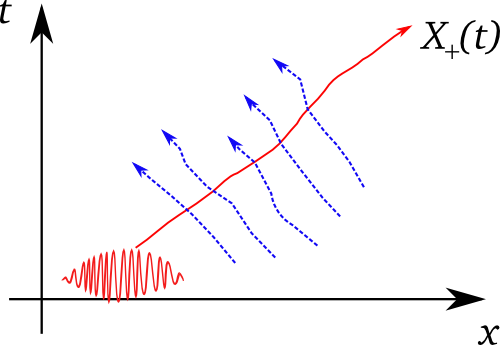
\includegraphics[width=0.8\columnwidth]{characteristics.png}
	\caption{The characteristic curve $X_{+}(t)$ giving the path of a right-moving phonon wavepacket is not straight due to the influence of the counterpropoagating waves.\trad{La courbe caractéristique \( X_{+}(t) \) donnant le chemin d'un paquet d'ondes phononiques se déplaçant vers la droite n'est pas droite en raison de l'influence des ondes se propageant dans la direction opposée.}}
	\label{fig:characteristics}
\end{figure}

It is natural to ask how this situation changes for a \emph{Fermi} gas, which has the hydrodynamic description 
%
\begin{equation}
	\label{GPEtoKPZ_FermiHydro}
	H_{\text{Fermi}}=  \int dx \left[\frac{\rho\left(\partial_{x} \theta\right)^{2}}{2m}+\frac{\pi^{2}\rho^{3}}{6m}\right],
\end{equation}
%
with the second term representing the Fermi pressure. The same analysis now yields the \emph{uncoupled} Burgers equations
%
\begin{equation}
	\label{GPEtoKPZ_FermiBurgers}
	\partial_{t}v_{\pm}+v_{\pm}\partial_{x}v_{\pm} =0
\end{equation}
%
where $v_{\pm}=v\pm \pi \rho/m$ are the right and left moving Fermi velocities. The characteristics $X_{\pm}(t)$ are now straight lines, and the free Fermi gas therefore represents an exceptional fluid in which we expect no anomalous broadening of the type discussed here.
\\
%(In general for $\mu\propto \rho^{\alpha}$, we have $v\pm \frac{2c}{\alpha}\left(\rho/\rho_{0}\right)^{\alpha/2}$)
\trad{
\emph{Équations du mouvement.} Pour obtenir une intuition sur la connexion entre l'équation de Gross-Pitaevskii (GPE) et l'équation de Burgers bruitée, puis à la classe de universalité KPZ, nous discutons des équations du mouvement du Hamiltonien donné par l'équation \eqref{GPEtoKPZ_HydroHam}. En ignorant le terme de pression quantique, celles-ci sont
%
\begin{equation*}
	%\label{GPEtoKPZ_HydroEq}
	\begin{split}
	\partial_{t} \rho+\partial_{x}\left(v\rho\right)=0	\\
	\partial_{t}v + v\partial_{x}v+(g/m)\partial_{x}\rho=0
	\end{split}
\end{equation*}
%
où \( v=\partial_{x}\theta/m \) est la vitesse superfluide. Ce sont les équations de continuité et d'Euler pour le gaz de Bose 1D, et peuvent être mises sous forme de Riemann \cite{Menikoff:1989}.
%
\begin{equation*}
	%\label{GPEtoKPZ_RHproblem}
	\partial_{t}(v\pm 2c_{\rho})+v_{\pm}\partial_{x}(v\pm 2c_{\rho})=0,
\end{equation*}
%
où \( v_{\pm}=v\pm c_{\rho} \), et \( c_{\rho}=c\sqrt{\rho/\rho_{0}} \) est la vitesse du son dans un référentiel où le fluide est localement au repos. L'équation \eqref{GPEtoKPZ_RHproblem} nous indique que \( v\pm 2c_{\rho} \) sont constants le long de leurs courbes caractéristiques respectives \( X_{\pm}(t) \) définies par \( \dot{X}_{\pm}(t)=v_{\pm}(X_{\pm}(t),t) \). Alternativement, nous pouvons écrire l'équation \eqref{GPEtoKPZ_RHproblem} comme
%
\begin{equation*}
	%\label{GPEtoKPZ_2Burgers}
	\partial_{t}v_{\pm}+v_{\pm}\partial_{x}v_{\pm}=\frac{1}{3}(\partial_{t}+v_{\pm}\partial_{x})v_{\mp}.
\end{equation*}
%
L'interprétation de l'équation \eqref{GPEtoKPZ_2Burgers} est la suivante. Les ondes sonores se déplaçant vers la droite et vers la gauche se propagent à travers le fluide à des vitesses \( v_{\pm} \), mais leur mouvement est perturbé par la variation dans le référentiel comove de la vitesse de l'onde qui se propage dans la direction opposée. En conséquence, les courbes caractéristiques ne sont pas des lignes droites (voir Fig.~\ref{fig:characteristics}). Nous pouvons considérer l'équation \eqref{GPEtoKPZ_2Burgers} comme une paire d'équations de Burgers entraînées, où les ondes se déplaçant vers la gauche agissent comme un terme de bruit sur la propagation des ondes se déplaçant vers la droite, et vice versa. Le terme visqueux \( \nu\partial_x^2v_{\pm} \) est absent pour ce système Hamiltonien mais sera généré lors du grossissement.
Il est naturel de se demander comment cette situation change pour un gaz de \emph{Fermi}, qui a la description hydrodynamique
%
\begin{equation*}
	%\label{GPEtoKPZ_FermiHydro}
	H_{\text{Fermi}}=  \int dx \left[\frac{\rho\left(\partial_{x} \theta\right)^{2}}{2m}+\frac{\pi^{2}\rho^{3}}{6m}\right],
\end{equation*}
%
où le deuxième terme représente la pression de Fermi. La même analyse donne maintenant les équations de Burgers \emph{découplées}
%
\begin{equation*}
	%\label{GPEtoKPZ_FermiBurgers}
	\partial_{t}v_{\pm}+v_{\pm}\partial_{x}v_{\pm} =0
\end{equation*}
%
où \( v_{\pm}=v\pm \pi \rho/m \) sont les vitesses de Fermi se déplaçant vers la droite et vers la gauche. Les caractéristiques \( X_{\pm}(t) \) sont maintenant des lignes droites, et le gaz de Fermi libre représente donc un fluide exceptionnel où nous ne nous attendons à aucune élargissement anomal de type discuté ici.
}
\\
\emph{Numerical simulations}. The GPE is solved using the splitting method, whereby $\Psi(x,t)$ is evolved for a timestep $\tau$ alternately by the kinetic $T=\frac{1}{2}\int dx\, |\partial_{x}\Psi|^{2}$ and potential $V=\frac{1}{2}\int\ dx\,|\Psi|^{4}$ terms of the Hamiltonian \cite{McLachlan:1993}
%
\begin{equation}
	\label{GPEtoKPZ_TVsplitting}
\begin{split}
	&\cT_{\tau}:\tilde\Psi(k,t)\to e^{-ik^{2}\tau/2}\tilde\Psi(k,t)\\
	&\cV_{\tau}:\Psi(x,t)\to e^{-i\tau|\Psi(x,t)|^{2}}\Psi(x,t),
\end{split}
\end{equation}
%
where $\tilde\Psi(k,t)$ denotes the Fourier transform of $\Psi(x,t)$, and we now switch to measuring distance in units of the healing length $\xi$, time in units of (inverse) chemical potential $\mu\equiv g\rho_{0}$, and $\Psi$ in units of $\sqrt{\rho_{0}}$. Algorithms of this type are \emph{symplectic}. This means that the method exactly simulates a Hamiltonian $H_{\tau}$ with $H_{\tau}-H$ a power series in $\tau$. The lowest power of $\tau$ in the series determines the \emph{order} of the method. Two benefits of symplectic integrators for statistical mechanical simulations are: i) exact conservation of phase space volume (i.e. Liouville's theorem is satisfied) and ii) no drift in the energy due to exact conservation of $H_{\tau}$.

We use the method $\cV_{\tau/2}\cdot\cT_{\tau}\cdot\cV_{\tau/2}$ -- often called `Leapfrog' -- which is second order with \cite{McLachlan:1993}
%
\begin{equation*}
	\label{GPEtoKPZ_Htau}
	\begin{split}
	H_{\tau}-H &= \frac{\tau^{2}}{24}\left(2\{T,\{V,T\}\}+\{V,\{T,V\}\}\right)+O(\tau^{4})\\
	&=\frac{\tau^{2}}{24}\int dx\left[\rho^{2}\left(\partial_{x}\theta\partial_{x}^{3}\theta-(\partial_{x}^{2}\theta)^{2}\right)-\rho(\partial_{x}\rho)^{2}\right]\\
	&\qquad\qquad+O(\tau^{4})		
	\end{split}
\end{equation*}
%
% For reference
% \begin{equation}
% 	\label{GPEtoKPZ_TVPBs}
% 	\begin{split}
% 	\left\{T,V\right\}&=-\frac{g}{m}\int dx\,\rho\partial_{x}\theta\partial_{x}\rho\\
% 	\left\{V,\left\{T,V\right\}\right\}&=-\frac{g^{2}}{m}\int dx\, \rho(\partial_{x}\rho)^{2}\\
% 	\left\{T,\left\{V,T\right\}\right\}&=\frac{g}{2m^{2}}\int dx\, \rho^{2}\left(\partial_{x}\theta\partial_{x}^{3}\theta-(\partial_{x}^{2}\theta)^{2}\right)
% 	\end{split}
% \end{equation}
We display the explicit form of the first correction term in $H_{\tau}$ to demonstrate that the additional terms generated by discretizing time are higher order in spatial gradients than Eq.~\eqref{GPEtoKPZ_CubicVertex}, and are therefore not expected to change the low $k$ behavior.

% TODO Symplectic integrator \cite{McLachlan:1993}
% TODO Initial conditions by equipartitition 

The harmonic modes are initially populated according to equipartition, so that the $\bop_{k}$ are taken as complex Gaussian random variables with $\langle|\bop_{k}|^{2}\rangle=\frac{T}{\cE_{k}}$ for temperature $T$. This assumes sufficiently weak nonlinearity, which is confirmed by the absence of transient behavior for the parameter ranges explored, indicating that the initial state is close to thermal.

We choose a spatial discretization scale $a=5$ to ensure all wavevectors are in the regime of linear dispersion $k\ll \xi^{-1}$. The time step of $\tau=2$ is then at the limit of stability of the algorithm. Most simulations use systems of length $L=2^{13}a$, but we check that the results are not significantly altered for $L=2^{14}a$ (see Fig.~\ref{fig:widths}). Periodic boundary conditions are used throughout.

At each time step we compute the Fourier components of the density $\rho(x,t)$
%
\begin{equation}
	\label{GPEtoKPZ_rhoq}
	\rho_{k}(t) = \sum_{n=0}^{N-1} |\Psi(na,t)|^{2}e^{-2\pi i kna}\qquad k = 0,\frac{2\pi}{L},\ldots, \frac{\pi}{a}.
\end{equation}
%
The resulting time series is then Fourier transformed to give the dynamical structure factor
%
\begin{equation}
	\label{GPEtoKPZ_StructureFactor}
	S(k,\omega)=\langle |\rho_{k,\omega}|^{2}\rangle, \qquad \omega = 0,\pm\frac{2\pi}{N_{\text{bin}}\tau},\ldots
\end{equation}
%
where $N_{\text{bin}}$ is the bin size used for the computation of the power spectra (at least $2^{20}$), and the angular brackets denotes an average over  $\sim 128$ runs of length $N_{\text{steps}}\tau$ with different random initial conditions. Thus for $N_{\text{bin}}=2^{20}$,  $N_{\text{steps}}=2^{21}$  corresponds to an effective average over $\sim 256$ runs, assuming no correlation between the two halves of a given run. 

We gather data for wavevectors $k=\frac{2\pi p}{L}$, with $p=1,2, 4,\ldots 4096$. Typical results, displaying good data collapse (assuming a width scaling as $|k|^{3/2}$) are shown in Fig.~\ref{fig:Lineshape}. For an unbiased test, power spectra are folded assuming symmetry between positive and negative frequencies, and the phonon peaks fitted to a Lorentzian to extract the amplitude, peak frequency, and width. Data are shown in Fig.~\ref{fig:widths}. A good fit to the scaling form $\Gamma_{k}\propto |k|^{z}$ is obtained over 1.5 decades and yields $z = 1.510 \pm 0.018$. Significant deviations from scaling are obtained at higher wavevectors.


%Absence of Rayleigh peaks in this simulation since $\gamma=1$

%Emphasize inapplicability of Golden Rule. Strictly linear phonons give infinite answer; allowing for curvature gives zero. Use Mazets as straw man? \cite{Mazets:2011}

\begin{figure}
	\centering
		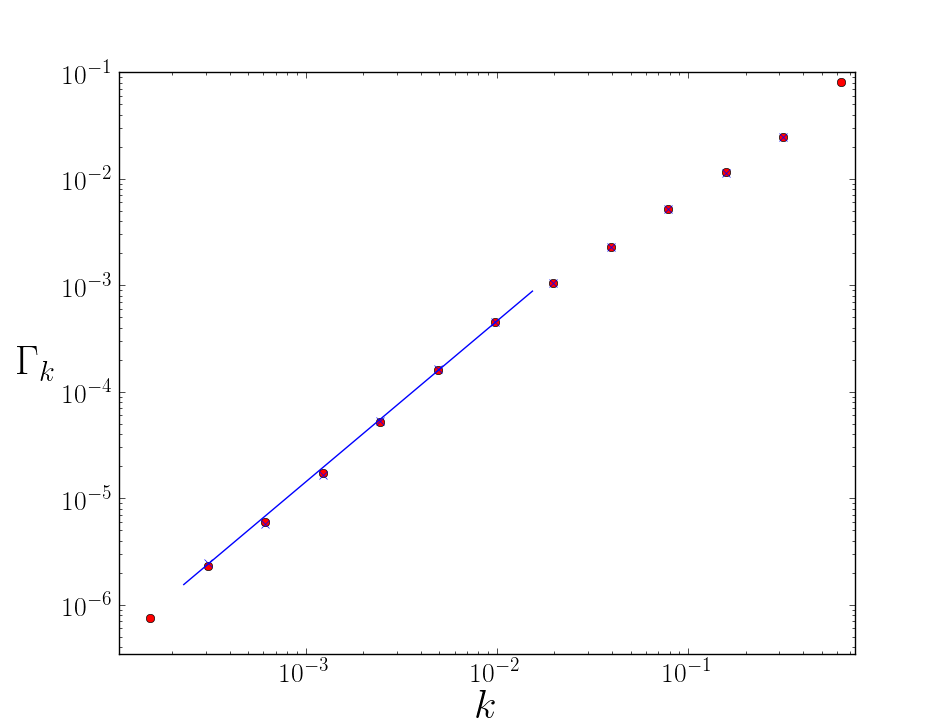
\includegraphics[width=\columnwidth]{WidthFit.png}
	\caption{Dependence of linewidth on wavevector, for system sizes $N=2^{13}$ (red dots) and $N=2^{14}$ (blue crosses), with $T=0.005$. The data are almost perfectly coincident. %\texttt{Dec 26 and Dec29 data for $N=2^{13}$ and $N=2^{14}$}. 
	The blue line is a fit for wavevectors $2\pi p / L$, $p=2,4,\ldots 64$ giving $z = 1.510 \pm 0.018$. %Inset: temperature dependence, \texttt{or measurement of sound velocity?}
	Higher wavevectors show a marked deviation from $3/2$ scaling, and $k=2\pi/L$ is omitted because the linewidth lies below resolution.
	\trad{Dépendance de la largeur de ligne en fonction du vecteur d'onde, pour des tailles de système \( N=2^{13} \) (points rouges) et \( N=2^{14} \) (croix bleues), avec \( T=0.005 \). Les données sont presque parfaitement coincidentes. %\texttt{Déc 26 et Déc 29 données pour \( N=2^{13} \) et \( N=2^{14} \)}.
	La ligne bleue est un ajustement pour les vecteurs d'ondes \( 2\pi p / L \), \( p=2,4,\ldots 64 \) donnant \( z = 1.510 \pm 0.018 \). %Inset : dépendance de la température, \texttt{ou mesure de la vitesse du son ?}
	Les vecteurs d'ondes plus élevés montrent un écart marqué par rapport à l'échelle \( 3/2 \), et \( k=2\pi/L \) est omis car la largeur de ligne est en dessous de la résolution.}
	}
	\label{fig:widths}
\end{figure}

%Further they would give the same answer for any system of waves with cubic nonlinearity, while the results of Ref.~\cite{narayan:2002} imply that Galilean invariance is essential for $z=3/2$. \texttt{Interesting question: how does the convective nonlinearity appear when you write waves on a chain?}

% TODO Fit tail to see PS behavior. As for Delfini mode coupling, the power is $\omega^{-7/3}$ (see Eq. 5.11 of Ref.~\cite{prahofer2004})

% TODO Errors in time discretization are higher derivative terms

% TODO Criterion to be at high temperature. When are quantum effects negligible?

% TODO Check at least two different sizes
% TODO At least two different temperatures
% TODO Pictures of scaling collapse of structure factor

% TODO Can we measure something analogous to the height distribution? e.g. phase distribution? This is relevant to split 1D condensatess

% TODO Picture in terms of characteristics, euler equations

\trad{
\emph{Simulations numériques}. L'équation de Gross-Pitaevskii (GPE) est résolue en utilisant la méthode de séparation, où \( \Psi(x,t) \) est évolué pour un pas de temps \( \tau \) alternativement par les termes cinétiques \( T = \frac{1}{2}\int dx\, |\partial_{x}\Psi|^{2} \) et potentiels \( V = \frac{1}{2}\int dx\,|\Psi|^{4} \) du Hamiltonien \cite{McLachlan:1993}
%
\begin{equation*}
	%\label{GPEtoKPZ_TVsplitting}
\begin{split}
	&\cT_{\tau}:\tilde\Psi(k,t)\to e^{-ik^{2}\tau/2}\tilde\Psi(k,t)\\
	&\cV_{\tau}:\Psi(x,t)\to e^{-i\tau|\Psi(x,t)|^{2}}\Psi(x,t),
\end{split}
\end{equation*}
%
où \( \tilde\Psi(k,t) \) désigne la transformation de Fourier de \( \Psi(x,t) \), et nous passons maintenant à mesurer la distance en unités de la longueur de guérison \( \xi \), le temps en unités de (inverse) du potentiel chimique \( \mu \equiv g\rho_{0} \), et \( \Psi \) en unités de \( \sqrt{\rho_{0}} \). Les algorithmes de ce type sont \emph{symplectiques}. Cela signifie que la méthode simule exactement un Hamiltonien \( H_{\tau} \) avec \( H_{\tau}-H \) étant une série en puissance de \( \tau \). La plus basse puissance de \( \tau \) dans la série détermine l'\emph{ordre} de la méthode. Deux avantages des intégrateurs symplectiques pour les simulations mécaniques statistiques sont : i) conservation exacte du volume de l'espace des phases (c'est-à-dire que le théorème de Liouville est satisfait) et ii) pas de dérive dans l'énergie en raison de la conservation exacte de \( H_{\tau} \).
Nous utilisons la méthode \( \cV_{\tau/2}\cdot\cT_{\tau}\cdot\cV_{\tau/2} \) — souvent appelée `Leapfrog' — qui est de second ordre avec \cite{McLachlan:1993}
%
\begin{equation*}
	%\label{GPEtoKPZ_Htau}
	\begin{split}
	H_{\tau}-H &= \frac{\tau^{2}}{24}\left(2\{T,\{V,T\}\}+\{V,\{T,V\}\}\right)+O(\tau^{4})\\
	&=\frac{\tau^{2}}{24}\int dx\left[\rho^{2}\left(\partial_{x}\theta\partial_{x}^{3}\theta-(\partial_{x}^{2}\theta)^{2}\right)-\rho(\partial_{x}\rho)^{2}\right]\\
	&\qquad\qquad+O(\tau^{4})		
	\end{split}
\end{equation*}
%
Nous affichons la forme explicite du premier terme de correction dans \( H_{\tau} \) pour démontrer que les termes supplémentaires générés par la discrétisation du temps sont de degré plus élevé en gradients spatiaux que l'équation \eqref{GPEtoKPZ_CubicVertex}, et ne sont donc pas censés modifier le comportement pour faible \( k \).
% TODO Intégrateur symplectique \cite{McLachlan:1993}
% TODO Conditions initiales par répartition de l'énergie
Les modes harmoniques sont initialement peuplés selon la répartition de l'énergie, de sorte que les \( \bop_{k} \) sont considérés comme des variables aléatoires gaussiennes complexes avec \( \langle|\bop_{k}|^{2}\rangle=\frac{T}{\cE_{k}} \) pour une température \( T \). Cela suppose une non-linéarité suffisamment faible, ce qui est confirmé par l'absence de comportement transitoire pour les plages de paramètres explorées, indiquant que l'état initial est proche de l'état thermique.
Nous choisissons une échelle de discrétisation spatiale \( a=5 \) pour garantir que tous les vecteurs d'ondes se trouvent dans le régime de dispersion linéaire \( k \ll \xi^{-1} \). Le pas de temps de \( \tau=2 \) est alors à la limite de stabilité de l'algorithme. La plupart des simulations utilisent des systèmes de longueur \( L=2^{13}a \), mais nous vérifions que les résultats ne sont pas significativement modifiés pour \( L=2^{14}a \) (voir Fig.~\ref{fig:widths}). Des conditions aux limites périodiques sont utilisées tout au long.
À chaque pas de temps, nous calculons les composants de Fourier de la densité \( \rho(x,t) \)
%
\begin{equation*}
	%\label{GPEtoKPZ_rhoq}
	\rho_{k}(t) = \sum_{n=0}^{N-1} |\Psi(na,t)|^{2}e^{-2\pi i kna}\qquad k = 0,\frac{2\pi}{L},\ldots, \frac{\pi}{a}.
\end{equation*}
%
La série temporelle résultante est ensuite transformée de Fourier pour donner le facteur de structure dynamique
%
\begin{equation}
	\label{GPEtoKPZ_StructureFactor}
	S(k,\omega)=\langle |\rho_{k,\omega}|^{2}\rangle, \qquad \omega = 0,\pm\frac{2\pi}{N_{\text{bin}}\tau},\ldots
\end{equation}
%
où \( N_{\text{bin}} \) est la taille des bins utilisée pour le calcul des spectres de puissance (au moins \( 2^{20} \)), et les crochets angulaires désignent une moyenne sur \( \sim 128 \) réalisations de longueur \( N_{\text{steps}}\tau \) avec des conditions initiales aléatoires différentes. Ainsi, pour \( N_{\text{bin}}=2^{20} \), \( N_{\text{steps}}=2^{21} \) correspond à une moyenne efficace sur \( \sim 256 \) réalisations, en supposant aucune corrélation entre les deux moitiés d'une réalisation donnée.
Nous recueillons des données pour les vecteurs d'ondes \( k = \frac{2\pi p}{L} \), avec \( p=1,2, 4,\ldots 4096 \). Les résultats typiques, montrant une bonne convergence des données (en supposant une largeur évoluant comme \( |k|^{3/2} \)), sont présentés dans la Fig.~\ref{fig:Lineshape}. Pour un test non biaisé, les spectres de puissance sont repliés en supposant une symétrie entre les fréquences positives et négatives, et les pics de phonons sont ajustés à une Lorentzienne pour extraire l'amplitude, la fréquence du pic et la largeur. Les données sont montrées dans la Fig.~\ref{fig:widths}. Un bon ajustement à la forme de mise à l'échelle \( \Gamma_{k}\propto |k|^{z} \) est obtenu sur 1,5 décades et donne \( z = 1.510 \pm 0.018 \). Des écarts significatifs par rapport à l'échelle sont obtenus pour des vecteurs d'ondes plus élevés.
%Absence de pics Rayleigh dans cette simulation puisque \( \gamma=1 \)
%Soulignez l'inapplicabilité de la Règle d'Or. Les phonons strictement linéaires donnent une réponse infinie ; permettre la courbure donne zéro. Utilisez Mazets comme straw man ? \cite{Mazets:2011}
%En outre, ils donneraient la même réponse pour tout système d'ondes avec non-linéarité cubique, tandis que les résultats de Ref.~\cite{narayan:2002} impliquent que l'invariance galiléenne est essentielle pour \( z=3/2 \). \texttt{Question intéressante : comment la non-linéarité convective apparaît-elle lorsque vous écrivez des ondes sur une chaîne ?}
% TODO Ajuster la queue pour voir le comportement PS. Comme pour le couplage des modes de Delfini, la puissance est \( \omega^{-7/3} \) (voir Eq. 5.11 de Ref.~\cite{prahofer2004})
% TODO Erreurs dans la discrétisation temporelle sont des termes de dérivées plus élevées
% TODO Critère pour être à haute température. Quand les effets quantiques sont-ils négligeables ?
% TODO Vérifier au moins deux tailles différentes
% TODO Au moins deux températures différentes
% TODO Images de la convergence des données du facteur de structure
% TODO Pouvons-nous mesurer quelque chose d'analogique à la distribution de hauteur ? Par exemple, distribution de phase ? Ceci est pertinent pour diviser les condensats 1D
% TODO Image en termes de caractéristiques, équations d'Euler
}\\

\emph{Conclusion}. We have provided convincing analytical and experimental evidence of the relationship between the finite temperature dynamics of the 1D Bose gas and the KPZ universality class. Galilean invariance is of paramount importance: simulations of wave equations with cubic nonlinearity but without Galilean invariance show $z\sim 1$ \cite{Kulkarni:}. Numerous extensions of the results of this work to multicomponent (or spinor) quantum fluids, and to transient rather than equilibrium dynamics, may be envisaged. In addition, the challenging problem of describing -- within a single framework -- the finite temperature phenomena described here, and the zero temperature results reviewed in Ref.~\cite{Imambekov:2011}, remains to be solved.
\trad{\emph{Conclusion}. Nous avons fourni des preuves analytiques et expérimentales convaincantes de la relation entre la dynamique à température finie du gaz de Bose 1D et la classe de l'universalité KPZ. L'invariance galiléenne est d'une importance capitale : les simulations d'équations d'ondes avec une non-linéarité cubique mais sans invariance galiléenne montrent \( z \sim 1 \) \cite{Kulkarni:}. De nombreuses extensions des résultats de ce travail aux fluides quantiques multicomposants (ou spinoriels), et à la dynamique transitoire plutôt qu'à l'équilibre, peuvent être envisagées. De plus, le problème difficile de décrire — dans un cadre unique — les phénomènes à température finie décrits ici, et les résultats à zéro température examinés dans la Ref.~\cite{Imambekov:2011}, reste à résoudre.
}\\
%Mention Extensions to spinor cases and relation to more than one interface models. 


\emph{Acknowledgements} Our thanks are due to Robert McLachlan and Uwe T\"auber for helpful discussions, and to the University of Virginia Alliance for Computational Science and Engineering, especially Katherine Holcomb, for their assistance. A.L. gratefully acknowledges the support of the Research Corporation and the NSF through award DMR-0846788. M.K thanks Saul Lapidus for useful discussions.
\trad{\emph{Acknowledgements}. Our thanks are due to Robert McLachlan and Uwe T\"auber for helpful discussions, and to the University of Virginia Alliance for Computational Science and Engineering, especially Katherine Holcomb, for their assistance. A.L. gratefully acknowledges the support of the Research Corporation and the NSF through award DMR-0846788. M.K. thanks Saul Lapidus for useful discussions.
}

%\bibliography{../Literature/1Dint}

%merlin.mbs apsrev4-1.bst 2010-07-25 4.21a (PWD, AO, DPC) hacked
%Control: key (0)
%Control: author (8) initials jnrlst
%Control: editor formatted (1) identically to author
%Control: production of article title (-1) disabled
%Control: page (0) single
%Control: year (1) truncated
%Control: production of eprint (0) enabled
\begin{thebibliography}{28}%
\makeatletter
\providecommand \@ifxundefined [1]{%
 \@ifx{#1\undefined}
}%
\providecommand \@ifnum [1]{%
 \ifnum #1\expandafter \@firstoftwo
 \else \expandafter \@secondoftwo
 \fi
}%
\providecommand \@ifx [1]{%
 \ifx #1\expandafter \@firstoftwo
 \else \expandafter \@secondoftwo
 \fi
}%
\providecommand \natexlab [1]{#1}%
\providecommand \enquote  [1]{``#1''}%
\providecommand \bibnamefont  [1]{#1}%
\providecommand \bibfnamefont [1]{#1}%
\providecommand \citenamefont [1]{#1}%
\providecommand \href@noop [0]{\@secondoftwo}%
\providecommand \href [0]{\begingroup \@sanitize@url \@href}%
\providecommand \@href[1]{\@@startlink{#1}\@@href}%
\providecommand \@@href[1]{\endgroup#1\@@endlink}%
\providecommand \@sanitize@url [0]{\catcode `\\12\catcode `\$12\catcode
  `\&12\catcode `\#12\catcode `\^12\catcode `\_12\catcode `\%12\relax}%
\providecommand \@@startlink[1]{}%
\providecommand \@@endlink[0]{}%
\providecommand \url  [0]{\begingroup\@sanitize@url \@url }%
\providecommand \@url [1]{\endgroup\@href {#1}{\urlprefix }}%
\providecommand \urlprefix  [0]{URL }%
\providecommand \Eprint [0]{\href }%
\providecommand \doibase [0]{http://dx.doi.org/}%
\providecommand \selectlanguage [0]{\@gobble}%
\providecommand \bibinfo  [0]{\@secondoftwo}%
\providecommand \bibfield  [0]{\@secondoftwo}%
\providecommand \translation [1]{[#1]}%
\providecommand \BibitemOpen [0]{}%
\providecommand \bibitemStop [0]{}%
\providecommand \bibitemNoStop [0]{.\EOS\space}%
\providecommand \EOS [0]{\spacefactor3000\relax}%
\providecommand \BibitemShut  [1]{\csname bibitem#1\endcsname}%
\let\auto@bib@innerbib\@empty
%</preamble>
\bibitem [{\citenamefont {Alder}\ and\ \citenamefont
  {Wainwright}(1970)}]{Alder:1970}%
  \BibitemOpen
  \bibfield  {author} {\bibinfo {author} {\bibfnamefont {B.}~\bibnamefont
  {Alder}}\ and\ \bibinfo {author} {\bibfnamefont {T.}~\bibnamefont
  {Wainwright}},\ }\href@noop {} {\bibfield  {journal} {\bibinfo  {journal}
  {Physical review A}\ }\textbf {\bibinfo {volume} {1}},\ \bibinfo {pages} {18}
  (\bibinfo {year} {1970})}\BibitemShut {NoStop}%
\bibitem [{\citenamefont {Ernst}\ \emph {et~al.}(1970)\citenamefont {Ernst},
  \citenamefont {Hauge},\ and\ \citenamefont {Van~Leeuwen}}]{Ernst:1970}%
  \BibitemOpen
  \bibfield  {author} {\bibinfo {author} {\bibfnamefont {M.}~\bibnamefont
  {Ernst}}, \bibinfo {author} {\bibfnamefont {E.}~\bibnamefont {Hauge}}, \ and\
  \bibinfo {author} {\bibfnamefont {J.}~\bibnamefont {Van~Leeuwen}},\
  }\href@noop {} {\bibfield  {journal} {\bibinfo  {journal} {Physical Review
  Letters}\ }\textbf {\bibinfo {volume} {25}},\ \bibinfo {pages} {1254}
  (\bibinfo {year} {1970})}\BibitemShut {NoStop}%
\bibitem [{\citenamefont {Dorfman}\ and\ \citenamefont
  {Cohen}(1970)}]{Dorfman:1970}%
  \BibitemOpen
  \bibfield  {author} {\bibinfo {author} {\bibfnamefont {J.}~\bibnamefont
  {Dorfman}}\ and\ \bibinfo {author} {\bibfnamefont {E.}~\bibnamefont
  {Cohen}},\ }\href@noop {} {\bibfield  {journal} {\bibinfo  {journal}
  {Physical Review Letters}\ }\textbf {\bibinfo {volume} {25}},\ \bibinfo
  {pages} {1257} (\bibinfo {year} {1970})}\BibitemShut {NoStop}%
\bibitem [{\citenamefont {Haldane}(1981)}]{Haldane:1981}%
  \BibitemOpen
  \bibfield  {author} {\bibinfo {author} {\bibfnamefont {F.}~\bibnamefont
  {Haldane}},\ }\href@noop {} {\bibfield  {journal} {\bibinfo  {journal}
  {Journal of Physics C: Solid State Physics}\ }\textbf {\bibinfo {volume}
  {14}},\ \bibinfo {pages} {2585} (\bibinfo {year} {1981})}\BibitemShut
  {NoStop}%
\bibitem [{\citenamefont {Giamarchi}(2004)}]{Giamarchi:2004}%
  \BibitemOpen
  \bibfield  {author} {\bibinfo {author} {\bibfnamefont {T.}~\bibnamefont
  {Giamarchi}},\ }\href@noop {} {\emph {\bibinfo {title} {Quantum physics in
  one dimension}}},\ Vol.\ \bibinfo {volume} {121}\ (\bibinfo  {publisher}
  {Oxford University Press, USA},\ \bibinfo {year} {2004})\BibitemShut
  {NoStop}%
\bibitem [{\citenamefont {Imambekov}\ \emph {et~al.}(2011)\citenamefont
  {Imambekov}, \citenamefont {Schmidt},\ and\ \citenamefont
  {Glazman}}]{Imambekov:2011}%
  \BibitemOpen
  \bibfield  {author} {\bibinfo {author} {\bibfnamefont {A.}~\bibnamefont
  {Imambekov}}, \bibinfo {author} {\bibfnamefont {T.}~\bibnamefont {Schmidt}},
  \ and\ \bibinfo {author} {\bibfnamefont {L.}~\bibnamefont {Glazman}},\
  }\href@noop {} {\bibfield  {journal} {\bibinfo  {journal} {Arxiv preprint
  arXiv:1110.1374}\ } (\bibinfo {year} {2011})}\BibitemShut {NoStop}%
\bibitem [{\citenamefont {Aristov}(2007)}]{Aristov:2007}%
  \BibitemOpen
  \bibfield  {author} {\bibinfo {author} {\bibfnamefont {D.}~\bibnamefont
  {Aristov}},\ }\href@noop {} {\bibfield  {journal} {\bibinfo  {journal}
  {Physical Review B}\ }\textbf {\bibinfo {volume} {76}},\ \bibinfo {pages}
  {085327} (\bibinfo {year} {2007})}\BibitemShut {NoStop}%
\bibitem [{\citenamefont {Cheianov}(2009)}]{Cheianov:2009}%
  \BibitemOpen
  \bibfield  {author} {\bibinfo {author} {\bibfnamefont {V.}~\bibnamefont
  {Cheianov}},\ }\href@noop {} {\bibfield  {journal} {\bibinfo  {journal}
  {Science}\ }\textbf {\bibinfo {volume} {323}},\ \bibinfo {pages} {213}
  (\bibinfo {year} {2009})}\BibitemShut {NoStop}%
\bibitem [{\citenamefont {Forster}(1975)}]{Forster:1975}%
  \BibitemOpen
  \bibfield  {author} {\bibinfo {author} {\bibfnamefont {D.}~\bibnamefont
  {Forster}},\ }\href@noop {} {\emph {\bibinfo {title} {Hydrodynamic
  fluctuations, broken symmetry, and correlation functions}}}\ (\bibinfo
  {publisher} {WA Benjamin, Inc., Reading, MA},\ \bibinfo {year}
  {1975})\BibitemShut {NoStop}%
\bibitem [{\citenamefont {van Beijeren}(2011)}]{beijeren2011}%
  \BibitemOpen
  \bibfield  {author} {\bibinfo {author} {\bibfnamefont {H.}~\bibnamefont {van
  Beijeren}},\ }\href@noop {} {\bibfield  {journal} {\bibinfo  {journal} {Arxiv
  preprint arXiv:1106.3298}\ } (\bibinfo {year} {2011})}\BibitemShut {NoStop}%
\bibitem [{\citenamefont {Kardar}\ \emph {et~al.}(1986)\citenamefont {Kardar},
  \citenamefont {Parisi},\ and\ \citenamefont {Zhang}}]{Kardar:1986}%
  \BibitemOpen
  \bibfield  {author} {\bibinfo {author} {\bibfnamefont {M.}~\bibnamefont
  {Kardar}}, \bibinfo {author} {\bibfnamefont {G.}~\bibnamefont {Parisi}}, \
  and\ \bibinfo {author} {\bibfnamefont {Y.}~\bibnamefont {Zhang}},\
  }\href@noop {} {\bibfield  {journal} {\bibinfo  {journal} {Physical Review
  Letters}\ }\textbf {\bibinfo {volume} {56}},\ \bibinfo {pages} {889}
  (\bibinfo {year} {1986})}\BibitemShut {NoStop}%
\bibitem [{\citenamefont {Kriecherbauer}\ and\ \citenamefont
  {Krug}(2010)}]{kriecherbauer2010}%
  \BibitemOpen
  \bibfield  {author} {\bibinfo {author} {\bibfnamefont {T.}~\bibnamefont
  {Kriecherbauer}}\ and\ \bibinfo {author} {\bibfnamefont {J.}~\bibnamefont
  {Krug}},\ }\href@noop {} {\bibfield  {journal} {\bibinfo  {journal} {Journal
  of Physics A: Mathematical and Theoretical}\ }\textbf {\bibinfo {volume}
  {43}},\ \bibinfo {pages} {403001} (\bibinfo {year} {2010})}\BibitemShut
  {NoStop}%
\bibitem [{\citenamefont {Sasamoto}\ and\ \citenamefont
  {Spohn}(2010)}]{sasamoto2010}%
  \BibitemOpen
  \bibfield  {author} {\bibinfo {author} {\bibfnamefont {T.}~\bibnamefont
  {Sasamoto}}\ and\ \bibinfo {author} {\bibfnamefont {H.}~\bibnamefont
  {Spohn}},\ }\href@noop {} {\bibfield  {journal} {\bibinfo  {journal} {Journal
  of Statistical Mechanics: Theory and Experiment}\ }\textbf {\bibinfo {volume}
  {2010}},\ \bibinfo {pages} {P11013} (\bibinfo {year} {2010})}\BibitemShut
  {NoStop}%
\bibitem [{\citenamefont {Pr\"ahofer}\ and\ \citenamefont
  {Spohn}(2004)}]{prahofer2004}%
  \BibitemOpen
  \bibfield  {author} {\bibinfo {author} {\bibfnamefont {M.}~\bibnamefont
  {Pr\"ahofer}}\ and\ \bibinfo {author} {\bibfnamefont {H.}~\bibnamefont
  {Spohn}},\ }\href@noop {} {\bibfield  {journal} {\bibinfo  {journal} {Journal
  of statistical physics}\ }\textbf {\bibinfo {volume} {115}},\ \bibinfo
  {pages} {255} (\bibinfo {year} {2004})}\BibitemShut {NoStop}%
\bibitem [{\citenamefont {Wakita}\ \emph {et~al.}(1997)\citenamefont {Wakita},
  \citenamefont {Itoh}, \citenamefont {Matsuyama},\ and\ \citenamefont
  {Matsushita}}]{wakita1997}%
  \BibitemOpen
  \bibfield  {author} {\bibinfo {author} {\bibfnamefont {J.}~\bibnamefont
  {Wakita}}, \bibinfo {author} {\bibfnamefont {H.}~\bibnamefont {Itoh}},
  \bibinfo {author} {\bibfnamefont {T.}~\bibnamefont {Matsuyama}}, \ and\
  \bibinfo {author} {\bibfnamefont {M.}~\bibnamefont {Matsushita}},\
  }\href@noop {} {\bibfield  {journal} {\bibinfo  {journal} {Journal of the
  Physical Society of Japan}\ }\textbf {\bibinfo {volume} {66}},\ \bibinfo
  {pages} {67} (\bibinfo {year} {1997})}\BibitemShut {NoStop}%
\bibitem [{\citenamefont {Maunuksela}\ \emph {et~al.}(1997)\citenamefont
  {Maunuksela}, \citenamefont {Myllys}, \citenamefont {K{\"a}hk{\"o}nen},
  \citenamefont {Timonen}, \citenamefont {Provatas}, \citenamefont {Alava},\
  and\ \citenamefont {Ala-Nissila}}]{maunuksela1997}%
  \BibitemOpen
  \bibfield  {author} {\bibinfo {author} {\bibfnamefont {J.}~\bibnamefont
  {Maunuksela}}, \bibinfo {author} {\bibfnamefont {M.}~\bibnamefont {Myllys}},
  \bibinfo {author} {\bibfnamefont {O.}~\bibnamefont {K{\"a}hk{\"o}nen}},
  \bibinfo {author} {\bibfnamefont {J.}~\bibnamefont {Timonen}}, \bibinfo
  {author} {\bibfnamefont {N.}~\bibnamefont {Provatas}}, \bibinfo {author}
  {\bibfnamefont {M.}~\bibnamefont {Alava}}, \ and\ \bibinfo {author}
  {\bibfnamefont {T.}~\bibnamefont {Ala-Nissila}},\ }\href@noop {} {\bibfield
  {journal} {\bibinfo  {journal} {Physical review letters}\ }\textbf {\bibinfo
  {volume} {79}},\ \bibinfo {pages} {1515} (\bibinfo {year}
  {1997})}\BibitemShut {NoStop}%
\bibitem [{\citenamefont {Takeuchi}\ and\ \citenamefont
  {Sano}(2010)}]{takeuchi2010}%
  \BibitemOpen
  \bibfield  {author} {\bibinfo {author} {\bibfnamefont {K.}~\bibnamefont
  {Takeuchi}}\ and\ \bibinfo {author} {\bibfnamefont {M.}~\bibnamefont
  {Sano}},\ }\href@noop {} {\bibfield  {journal} {\bibinfo  {journal} {Physical
  review letters}\ }\textbf {\bibinfo {volume} {104}},\ \bibinfo {pages}
  {230601} (\bibinfo {year} {2010})}\BibitemShut {NoStop}%
\bibitem [{\citenamefont {Fabbri}\ \emph {et~al.}(2011)\citenamefont {Fabbri},
  \citenamefont {Cl\'ement}, \citenamefont {Fallani}, \citenamefont {Fort},\
  and\ \citenamefont {Inguscio}}]{Fabbri:2011}%
  \BibitemOpen
  \bibfield  {author} {\bibinfo {author} {\bibfnamefont {N.}~\bibnamefont
  {Fabbri}}, \bibinfo {author} {\bibfnamefont {D.}~\bibnamefont {Cl\'ement}},
  \bibinfo {author} {\bibfnamefont {L.}~\bibnamefont {Fallani}}, \bibinfo
  {author} {\bibfnamefont {C.}~\bibnamefont {Fort}}, \ and\ \bibinfo {author}
  {\bibfnamefont {M.}~\bibnamefont {Inguscio}},\ }\href {\doibase
  10.1103/PhysRevA.83.031604} {\bibfield  {journal} {\bibinfo  {journal} {Phys.
  Rev. A}\ }\textbf {\bibinfo {volume} {83}},\ \bibinfo {pages} {031604}
  (\bibinfo {year} {2011})}\BibitemShut {NoStop}%
\bibitem [{\citenamefont {Savard}\ \emph {et~al.}(2011)\citenamefont {Savard},
  \citenamefont {Dauphinais},\ and\ \citenamefont {Gervais}}]{savard2011}%
  \BibitemOpen
  \bibfield  {author} {\bibinfo {author} {\bibfnamefont {M.}~\bibnamefont
  {Savard}}, \bibinfo {author} {\bibfnamefont {G.}~\bibnamefont {Dauphinais}},
  \ and\ \bibinfo {author} {\bibfnamefont {G.}~\bibnamefont {Gervais}},\ }\href
  {\doibase 10.1103/PhysRevLett.107.254501} {\bibfield  {journal} {\bibinfo
  {journal} {Phys. Rev. Lett.}\ }\textbf {\bibinfo {volume} {107}},\ \bibinfo
  {pages} {254501} (\bibinfo {year} {2011})}\BibitemShut {NoStop}%
\bibitem [{\citenamefont {Andreev}(1980)}]{andreev:1980}%
  \BibitemOpen
  \bibfield  {author} {\bibinfo {author} {\bibfnamefont {A.}~\bibnamefont
  {Andreev}},\ }\href@noop {} {\bibfield  {journal} {\bibinfo  {journal}
  {Zhurnal Eksperimental noi i Teoreticheskoi Fiziki}\ }\textbf {\bibinfo
  {volume} {78}},\ \bibinfo {pages} {2064} (\bibinfo {year}
  {1980})}\BibitemShut {NoStop}%
\bibitem [{\citenamefont {Samokhin}(1998)}]{Samokhin:1998}%
  \BibitemOpen
  \bibfield  {author} {\bibinfo {author} {\bibfnamefont {K.}~\bibnamefont
  {Samokhin}},\ }\href@noop {} {\bibfield  {journal} {\bibinfo  {journal}
  {Journal of Physics: Condensed Matter}\ }\textbf {\bibinfo {volume} {10}},\
  \bibinfo {pages} {L533} (\bibinfo {year} {1998})}\BibitemShut {NoStop}%
\bibitem [{\citenamefont {Delfini}\ \emph {et~al.}(2006)\citenamefont
  {Delfini}, \citenamefont {Lepri}, \citenamefont {Livi},\ and\ \citenamefont
  {Politi}}]{delfini2006}%
  \BibitemOpen
  \bibfield  {author} {\bibinfo {author} {\bibfnamefont {L.}~\bibnamefont
  {Delfini}}, \bibinfo {author} {\bibfnamefont {S.}~\bibnamefont {Lepri}},
  \bibinfo {author} {\bibfnamefont {R.}~\bibnamefont {Livi}}, \ and\ \bibinfo
  {author} {\bibfnamefont {A.}~\bibnamefont {Politi}},\ }\href@noop {}
  {\bibfield  {journal} {\bibinfo  {journal} {Physical Review E}\ }\textbf
  {\bibinfo {volume} {73}},\ \bibinfo {pages} {060201} (\bibinfo {year}
  {2006})}\BibitemShut {NoStop}%
\bibitem [{\citenamefont {Forster}\ \emph {et~al.}(1977)\citenamefont
  {Forster}, \citenamefont {Nelson},\ and\ \citenamefont
  {Stephen}}]{forster1977}%
  \BibitemOpen
  \bibfield  {author} {\bibinfo {author} {\bibfnamefont {D.}~\bibnamefont
  {Forster}}, \bibinfo {author} {\bibfnamefont {D.}~\bibnamefont {Nelson}}, \
  and\ \bibinfo {author} {\bibfnamefont {M.}~\bibnamefont {Stephen}},\
  }\href@noop {} {\bibfield  {journal} {\bibinfo  {journal} {Physical Review
  A}\ }\textbf {\bibinfo {volume} {16}},\ \bibinfo {pages} {732} (\bibinfo
  {year} {1977})}\BibitemShut {NoStop}%
\bibitem [{\citenamefont {Narayan}\ and\ \citenamefont
  {Ramaswamy}(2002)}]{narayan:2002}%
  \BibitemOpen
  \bibfield  {author} {\bibinfo {author} {\bibfnamefont {O.}~\bibnamefont
  {Narayan}}\ and\ \bibinfo {author} {\bibfnamefont {S.}~\bibnamefont
  {Ramaswamy}},\ }\href@noop {} {\bibfield  {journal} {\bibinfo  {journal}
  {Physical review letters}\ }\textbf {\bibinfo {volume} {89}},\ \bibinfo
  {pages} {200601} (\bibinfo {year} {2002})}\BibitemShut {NoStop}%
\bibitem [{\citenamefont {Frey}\ \emph {et~al.}(1996)\citenamefont {Frey},
  \citenamefont {T{\"a}uber},\ and\ \citenamefont {Hwa}}]{frey1996}%
  \BibitemOpen
  \bibfield  {author} {\bibinfo {author} {\bibfnamefont {E.}~\bibnamefont
  {Frey}}, \bibinfo {author} {\bibfnamefont {U.}~\bibnamefont {T{\"a}uber}}, \
  and\ \bibinfo {author} {\bibfnamefont {T.}~\bibnamefont {Hwa}},\ }\href@noop
  {} {\bibfield  {journal} {\bibinfo  {journal} {Physical Review E}\ }\textbf
  {\bibinfo {volume} {53}},\ \bibinfo {pages} {4424} (\bibinfo {year}
  {1996})}\BibitemShut {NoStop}%
\bibitem [{\citenamefont {Menikoff}\ and\ \citenamefont
  {Plohr}(1989)}]{Menikoff:1989}%
  \BibitemOpen
  \bibfield  {author} {\bibinfo {author} {\bibfnamefont {R.}~\bibnamefont
  {Menikoff}}\ and\ \bibinfo {author} {\bibfnamefont {B.~J.}\ \bibnamefont
  {Plohr}},\ }\href {\doibase 10.1103/RevModPhys.61.75} {\bibfield  {journal}
  {\bibinfo  {journal} {Rev. Mod. Phys.}\ }\textbf {\bibinfo {volume} {61}},\
  \bibinfo {pages} {75} (\bibinfo {year} {1989})}\BibitemShut {NoStop}%
\bibitem [{\citenamefont {McLachlan}(1993)}]{McLachlan:1993}%
  \BibitemOpen
  \bibfield  {author} {\bibinfo {author} {\bibfnamefont {R.}~\bibnamefont
  {McLachlan}},\ }\href@noop {} {\bibfield  {journal} {\bibinfo  {journal}
  {Numerische Mathematik}\ }\textbf {\bibinfo {volume} {66}},\ \bibinfo {pages}
  {465} (\bibinfo {year} {1993})}\BibitemShut {NoStop}%
\bibitem [{\citenamefont {Kulkarni}\ and\ \citenamefont
  {Lamacraft}()}]{Kulkarni:}%
  \BibitemOpen
  \bibfield  {author} {\bibinfo {author} {\bibfnamefont {M.}~\bibnamefont
  {Kulkarni}}\ and\ \bibinfo {author} {\bibfnamefont {A.}~\bibnamefont
  {Lamacraft}},\ }\href@noop {} {\bibinfo  {journal} {(Unpublished)}\
  }\BibitemShut {NoStop}%
\end{thebibliography}%


\end{document}